\documentclass[11pt,a4paper]{article}

\usepackage[margin=25mm]{geometry}
\usepackage{booktabs}
\usepackage{caption}
\usepackage{float}
\usepackage{graphicx}
\usepackage{hyperref}

\hypersetup{
    colorlinks=true,
    linkcolor=black,
    urlcolor=blue
}

\title{Adaptive Media Processing Assignment 2\\Fisher's Iris Classification Problem}
\author{}
\date{}

\begin{document}

\maketitle

\section{Source Code}

The full implementation of the classifiers, experiments, and result generation is provided in the Jupyter notebook \texttt{assignment\_2.ipynb}. The notebook contains the custom implementation of the k-nearest neighbor classifier and the Fisher linear discriminator used for this report. This PDF report includes the method descriptions, plots, results, and discussion, while excluding the source code itself.

\section{Solution}

As a first step, the classifiers were created and tested on one split of the dataset, using 50\% of the samples for training and the remaining 50\% for testing. The following metrics were used to evaluate performance: accuracy, precision, recall, F1-score, and the confusion matrix. This preliminary evaluation was used to validate the behavior of the classifiers before running the repeated experiment required by the assignment.

\subsection{KNN Classifier}

The k-nearest neighbor classifier identifies the \(k\) nearest neighbors of a given input \(X\). It does so by calculating the Euclidean distance between \(X\) and every sample in the training dataset. Once the nearest neighbors have been selected, each neighbor votes for its corresponding class, and the class with the highest number of votes is returned.

The classifier has two main steps. During fitting, all training inputs are stored together with their corresponding labels. No additional parameter estimation is required for KNN. During prediction, the \(k\) nearest neighbors are retrieved for each test sample, and the class with the highest vote count is returned.

Table~\ref{tab:knn-single-split} and Figure~\ref{fig:knn-confusion} show the performance of the KNN classifier on the preliminary split.

\begin{table}[H]
\centering
\caption{KNN classification report on the preliminary split.}
\label{tab:knn-single-split}
\begin{tabular}{lrrrr}
\toprule
Class & Precision & Recall & F1-score & Support \\
\midrule
Setosa & 1.00 & 1.00 & 1.00 & 21 \\
Versicolor & 0.96 & 0.89 & 0.92 & 27 \\
Virginica & 0.90 & 0.96 & 0.93 & 27 \\
\midrule
Accuracy & \multicolumn{3}{r}{0.95} & 75 \\
Macro average & 0.95 & 0.95 & 0.95 & 75 \\
Weighted average & 0.95 & 0.95 & 0.95 & 75 \\
\bottomrule
\end{tabular}
\end{table}

\begin{figure}[H]
\centering
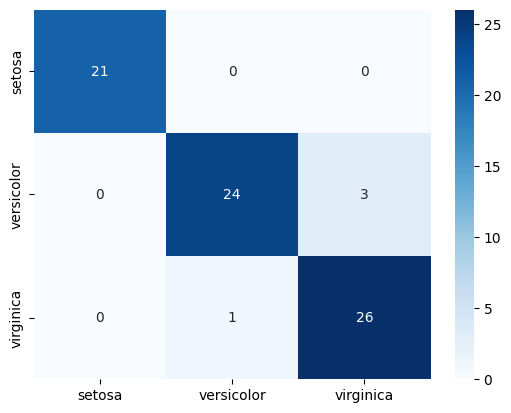
\includegraphics[width=0.68\textwidth]{figures/knn_confusion_matrix.png}
\caption{KNN confusion matrix on the preliminary split.}
\label{fig:knn-confusion}
\end{figure}

\subsection{Selection of k}

To select an appropriate value for \(k\), which is the main hyperparameter of this KNN implementation, the classifier was evaluated using values from 1 to 20. For each value, accuracy, precision, recall, and F1-score were calculated on the preliminary validation split. The value \(k = 6\) was selected because it produced the best overall result in this evaluation, particularly according to the accuracy curve.

\begin{figure}[H]
\centering
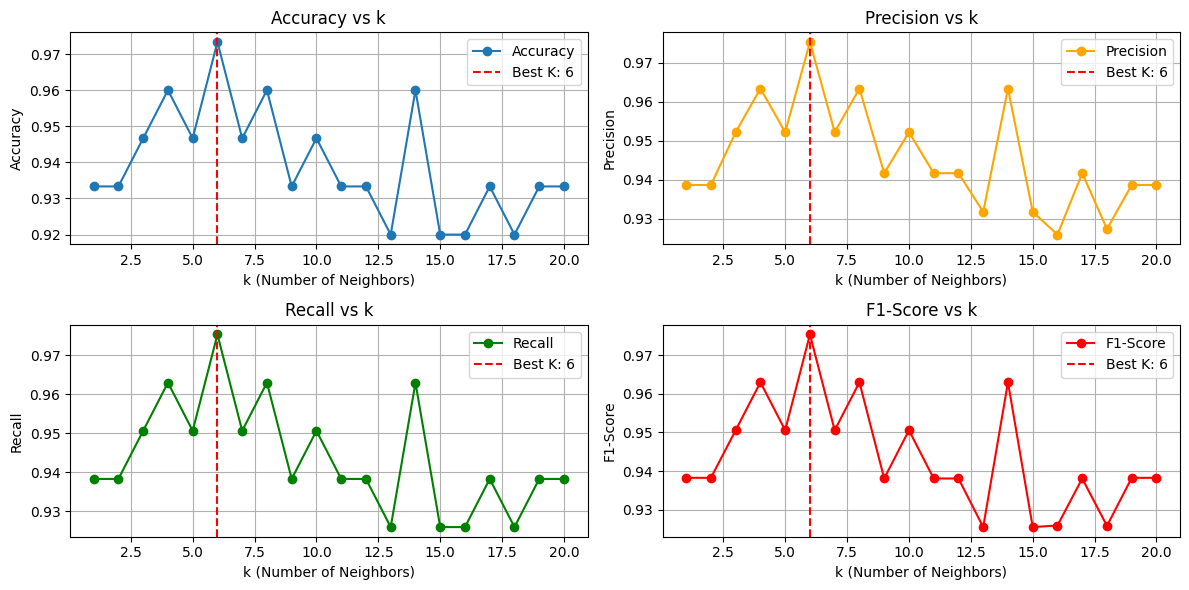
\includegraphics[width=\textwidth]{figures/knn_k_selection.png}
\caption{Evaluation of KNN performance for \(k\) values from 1 to 20.}
\label{fig:knn-k-selection}
\end{figure}

\subsection{Fisher Classifier}

The Fisher classifier was implemented using \(n\) binary classifiers based on Fisher's linear discriminator. In the Iris dataset, there are three classes: Setosa, Versicolor, and Virginica. Therefore, \(n = 3\), and three binary classifiers were created.

These classifiers were combined using a one-vs-rest approach. To determine which class best corresponds to an input \(X\), it is projected using the projection vector \(w\) of each classifier and compared with the corresponding threshold. Instead of using each threshold only to produce a binary decision, each classifier returns a score that represents how far the projected sample is from its decision boundary. The final predicted class is the one with the highest score.

Table~\ref{tab:fisher-single-split} and Figure~\ref{fig:fisher-confusion} show the performance of the Fisher classifier on the preliminary split.

\begin{table}[H]
\centering
\caption{Fisher classification report on the preliminary split.}
\label{tab:fisher-single-split}
\begin{tabular}{lrrrr}
\toprule
Class & Precision & Recall & F1-score & Support \\
\midrule
Setosa & 1.00 & 1.00 & 1.00 & 21 \\
Versicolor & 0.85 & 0.85 & 0.85 & 27 \\
Virginica & 0.85 & 0.85 & 0.85 & 27 \\
\midrule
Accuracy & \multicolumn{3}{r}{0.89} & 75 \\
Macro average & 0.90 & 0.90 & 0.90 & 75 \\
Weighted average & 0.89 & 0.89 & 0.89 & 75 \\
\bottomrule
\end{tabular}
\end{table}

\begin{figure}[H]
\centering
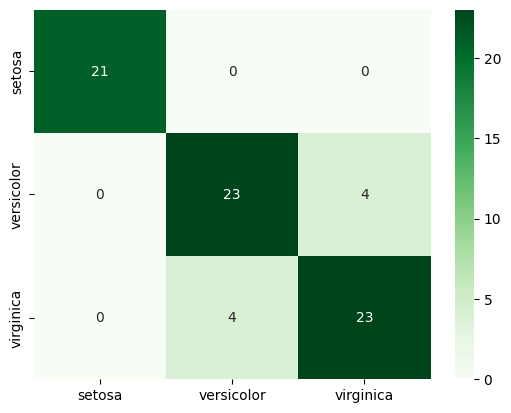
\includegraphics[width=0.68\textwidth]{figures/fisher_confusion_matrix.png}
\caption{Fisher classifier confusion matrix on the preliminary split.}
\label{fig:fisher-confusion}
\end{figure}

\section{Repeated Experiment Results}

Both \texttt{KNNClassifier} and \texttt{FisherClassifier} were then trained and evaluated according to the assignment instructions. The data was divided using stratified random splits so that each class was divided in half: 25 samples per class for training and 25 samples per class for testing. This random selection, training, and testing procedure was repeated 20 times.

Table~\ref{tab:overall-results} shows the overall classification performance across the 20 random splits. The reported values include the mean, variance, and standard deviation for accuracy, precision, recall, and F1-score.

\begin{table}[H]
\centering
\caption{Overall classification results across 20 stratified random splits.}
\label{tab:overall-results}
\resizebox{\textwidth}{!}{%
\begin{tabular}{lrrrrrrrrrrrr}
\toprule
Classifier & Acc. Mean & Acc. Var. & Acc. Std. & Prec. Mean & Prec. Var. & Prec. Std. & Rec. Mean & Rec. Var. & Rec. Std. & F1 Mean & F1 Var. & F1 Std. \\
\midrule
KNN    & 0.958 & 0.000 & 0.017 & 0.960 & 0.000 & 0.016 & 0.958 & 0.000 & 0.017 & 0.958 & 0.000 & 0.018 \\
Fisher & 0.859 & 0.002 & 0.042 & 0.866 & 0.002 & 0.044 & 0.859 & 0.002 & 0.042 & 0.858 & 0.002 & 0.043 \\
\bottomrule
\end{tabular}
}
\end{table}

Table~\ref{tab:class-results} shows the per-class precision, recall, and F1-score results. Accuracy is reported only for the overall classification rate, while the per-class rows provide class-specific precision, recall, and F1-score.

\begin{table}[H]
\centering
\caption{Per-class classification results across 20 stratified random splits.}
\label{tab:class-results}
\resizebox{\textwidth}{!}{%
\begin{tabular}{llrrrrrrrrr}
\toprule
Classifier & Class & Prec. Mean & Prec. Var. & Prec. Std. & Rec. Mean & Rec. Var. & Rec. Std. & F1 Mean & F1 Var. & F1 Std. \\
\midrule
KNN    & Setosa     & 1.000 & 0.000 & 0.000 & 1.000 & 0.000 & 0.000 & 1.000 & 0.000 & 0.000 \\
KNN    & Versicolor & 0.930 & 0.003 & 0.056 & 0.950 & 0.001 & 0.036 & 0.938 & 0.001 & 0.025 \\
KNN    & Virginica  & 0.951 & 0.001 & 0.034 & 0.924 & 0.004 & 0.065 & 0.935 & 0.001 & 0.028 \\
Fisher & Setosa     & 1.000 & 0.000 & 0.000 & 1.000 & 0.000 & 0.000 & 1.000 & 0.000 & 0.000 \\
Fisher & Versicolor & 0.834 & 0.009 & 0.096 & 0.736 & 0.008 & 0.091 & 0.776 & 0.005 & 0.068 \\
Fisher & Virginica  & 0.764 & 0.004 & 0.062 & 0.842 & 0.011 & 0.105 & 0.798 & 0.004 & 0.065 \\
\bottomrule
\end{tabular}
}
\end{table}

\section{Discussion}

After repeating the random train/test split 20 times, the k-nearest neighbor classifier achieved the highest overall performance, with an average accuracy of approximately 0.958. Its rounded accuracy variance is close to 0.000, indicating that its performance was also stable across the different random splits. The Fisher classifier obtained a lower average accuracy of approximately 0.859, with an accuracy variance of approximately 0.002.

The main reason for this difference is the way each classifier separates the data. KNN is a local method: it classifies each test example by considering nearby training examples. This approach works well for the Iris dataset because samples from the same species tend to form local groups in the feature space. Fisher's linear discriminator, on the other hand, projects the data onto linear decision directions. This makes the model simpler and more constrained, so it has more difficulty when two classes overlap or are not clearly separated by a linear boundary.

Both methods classify Iris Setosa almost perfectly because Setosa is clearly separated from the other two species. Most errors occur between Iris Versicolor and Iris Virginica. These two classes have more similar petal and sepal measurements, so their feature distributions overlap. This overlap affects the Fisher classifier more strongly, which explains its lower precision, recall, and F1-score for these two classes. KNN handles this overlap more effectively because it can adapt to the local structure of the samples instead of relying only on a global linear separation.

\end{document}
